\documentclass[../main.tex]{subfiles}
\graphicspath{{\subfix{../images/}}}
\begin{document}
\section{Complexité du problème du cycle Hamiltonien}
Le problème de décision: Est-ce que un graphe quelconque $G(V, A)$ contient un cycle Hamiltonien (un cycle qui passe par tout les sommets une seule fois)? est un problème important à étudier (dans un point de vue de complexité) pour classifier le TSP. Cette section prouvera cycle hamiltonien (\emph{HC}) est NP-complet. Pour cela, il suffit de vérifier 2 propriétés:

\begin{enumerate}
\item $HC \in$ NP.
\item Un problème NP-complet peut être réduit dans un temps polynomial à $HC$ (équivalent à dire que tout problème dans NP est réductible à $HC$).
\end{enumerate}

Pour prouver 1. il suffit de prouver qu'une solution (pour un graphe $G(V,A)$) donnée peut être vérifiée dans un temps polynomial. Une solution aura la forme d'un ensemble d'arêtes $S$, il faut alors vérifier 3 propriétés dans cette solution:

\begin{enumerate}
\item $|S| = |V|$
\item $\forall i \in S, \ i \in A$
\item $\forall v \in V$, $v$ apparaît seulement 2 fois dans $(a, b) \in S$. 
\end{enumerate}

Vu que toutes ces tâches augmentent avec un ordre proportionnel à $|V|$, une solution peut être vérifiée dans un temps polynomial.

Nous choisissons une réduction du problème de la \og Couverture de sommet \fg{} qui à été prouvée être NP-complet par \cite{Karp1972}. Tout simplement, une couverture de sommet pour un graphe $G(V,A)$ est un ensemble de sommets $S \subseteq V$, qui vérifie la propriété suivante:

\[
\forall (u,v) \in A, \ u \in S \lor v \in S
\]
Autrement dit, tout les arêtes sont incidents à au moins un sommet dans la couverture.

Le problème de la couverture de sommet dit: Soit un graphe $G(V,A)$ et un entier $K$, est-ce qu'il existe une couverture $S$ tel que $|S|\leq K$? Nous présentons alors cette réduction prise de \cite{Hartmanis1982}.

\subsection{Algorithme de réduction}
Le but est de transformer le graphe $G(V,A)$ en un graphe $G'(V', A')$ pour lequel il existera un cycle Hamiltonien dans $G'$ si et seulement si $G$ contient une couverture de sommet de taille au plus $K$. Cet algorithme transforme chaque arête $(u,v)\in A$ à une structure de 12 sommets et 14 arêtes (voir Figure \ref{fig:structure_hamiltonian}) définit comme
\begin{align*}
V_e' = &\{(u,e,i),(v,e,i): 1 \leq i \leq 6\}\\
A_e' = &\{((u, e, i), (u,e,i+1)), ((v, e, i), (v,e,i+1)): 1 \leq i \leq 5 \}\\
\cup &\{((u, e, 3), (v,e,1)), ((u, e, 1), (v,e,3))\}\\
\cup &\{((u, e, 6), (v,e,4)), ((u, e, 4), (v,e,6))\}
\end{align*}

\begin{figure}[!htb]
    \centering
    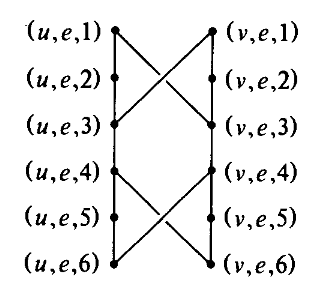
\includegraphics[scale=0.8]{structure_hamiltonian}
    \caption{Illustration de la structure}
    \label{fig:structure_hamiltonian}
\end{figure}


Le but de ces structures est de forcer n'importe quel cycle Hamiltonien de le traverser d'une des trois manières (voir Figure \ref{fig:possible_cycles}) . Il y aura alors autant de ces structures que le nombre d'arête dans le graphe original. Pour rappeler, chaque structure est associé à 2 sommets, il y a aura alors autant de structure pour un sommet que son degrés. Nous ordonnons arbitrairement les arêtes dans $G$ afin de nommer les sommets dans les structures comme $e_{v[1]},e_{v[2]},\dots, e_{v[deg(v)]}$ avec $deg(v)$ le degré du sommet $v$. Ces structures sont reliés ensemble avec les arête suivantes:
\[
A_v' = \{((v, e_{v[i]}, 6), (v, e_{v[i+1]}, 1)): 1 \leq i \leq deg(v)-1 \}
\]
Autrement dit, chaque structure sera reliée jusqu'à un maximum de 4 autres structures (2 pour chaque côté droite ou gauche).

\begin{figure}[!htb]
    \centering
    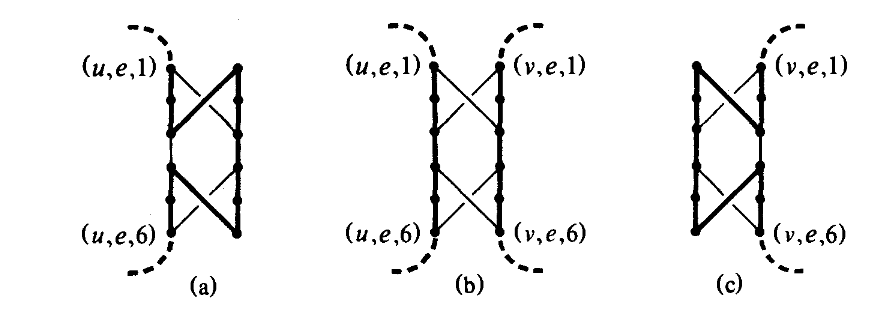
\includegraphics[scale=0.8]{possible_cycles}
    \caption{Les 3 cas possible pour un cycle Hamiltonien de passer à travers la structure. Cas (a) correspond au sommet $u \in S$ (la couverture), cas (b) correspond à $\{u,v\} \subseteq S$ et cas (c) correspond à $v \in S$}
    \label{fig:possible_cycles}
\end{figure}

Finalement l'algorithme ajoute $K$ sommets ($a_1, a_2, \dots a_k$) qui seront les \og sommets de sélection \fg{} et ils seront reliés à chaque début et fin d'une branche qui relie les \og chaînes \fg{} de sommets en commun ensemble. Formellement l'ensemble d'arête supplémentaire est définit comme:
\[
A'' = \{(a_i, (v, e_{v[1]}, 1)), (a_i, (v, e_{v[deg(v)]}, 6)): 1 \leq i \leq K, v \in V \}
\]  
Ce qui donne enfin un graphe $G'(V',A')$ tel que:
\begin{align*}
V' &= \{ a_i: 1 \leq i \leq K \} \cup \left( \bigcup_{e \in A} V_e' \right)\\
A' &= \left( \bigcup_{e \in A} A_e' \right) \cup \left( \bigcup_{v \in V} A_v' \right) \cup A''
\end{align*}

Il est important de noter que $G'$ peut être construit dans un temps polynomial à partir de $G$. La complexité en temps est proportionnelle au nombre d'arête dans le graphe + les arêtes qui relient $a_i$ aux structures, qui est proportionnel au nombre de sommets.

\subsection{Prouver la réduction}
Maintenant il suffit que la réduction présentée ci dessus soit bien une réduction. Autrement dit, il faut prouver que $G'$ contient un cycle Hamiltonien si et seulement si $G$ contient une couverture de taille $K$. Soit $<v_1, v_2, \dots , v_n>$ avec $n = |V'|$ est un cycle Hamiltonien pour $G'$. Prenons en considération une portion du cycle qui commence d'un des sommets sélecteurs $\{a_i: 1 \leq i \leq K \}$ et termine à un de ces vecteurs sans passer par un vecteur sélecteur entre les deux. Selon la Figure \ref{fig:possible_cycles}, si un cycle entre la structure par le côté $v$ il doit sortir à travers le côté $v$ (de même pour $u$). Alors cette portion de cycle traversera tous les structures associées avec un vecteur $v$. Le cycle Hamiltonien peut alors être divisé en $K$ portions chacune traversant un sommet $v$ différent.

Une couverture de taille $K$ est simplement l'ensemble de sommets adjacents aux sommets sélecteurs. Parce que le cycle est Hamiltonien (il passe par toutes les structures) et chaque portion du cycle passe par les arêtes adjacentes à un seul sommet $v$, la couverture spécifié auparavant est bien une couverture de $G$.

Dans un autre temps, soit $V^* \subseteq V$ une couverture de taille au plus $K$. Nous pouvons supposer que $|V^*| = K$ car ajouter des vecteurs supplémentaire à l'ensemble reste quand même une couverture, soit $V^* = \{v_1, v_2, \dots , v_k \}$. La somme des arêtes suivants formeront un cycle Hamiltonien pour $G'$. Pour la structure illustrée par la Figure \ref{fig:structure_hamiltonian}, les arêtes de la Figure \ref{fig:possible_cycles} (cas (a), (b) ou (c)) sont choisi selon le résultat de $\{u ,v\} \cap V^*$: $\{u\}$ prendra le cas (a), $\{u,v\}$ prendra le cas (b) et $\{v\}$ prendra le cas (c). Il est important de noter que le résultat $\emptyset$ est impossible car $V^*$ est une couverture et alors il doit avoir au moins un sommet adjacent de $V^*$.

Ensuite il faut choisir les arêtes $E_{v_i}$ pour $1 \leq i \leq K$ (les arêtes qui relient les structures des sommets sélecteurs) et aussi
\[
\{a_i, (v_i, e_{v_i[1]}, 1) \}, 1 \leq i \leq K
\]
et
\[
\{a_{i+1}, (v_i, e_{v_i[deg(v_i)]}, 6 )\}, 1 \leq i \leq K -1
\]
et enfin
\[
\{a_1, (v_K, e_{v_K[deg(v_K)]}, 6 )\}
\]

Ce cycle est Hamiltonien. Alors le problème de couverture des sommets peut être réduit au problème du cycle Hamiltonien, qui est en NP. Par la suite le problème du cycle Hamiltonien est un problème NP-complet.

\end{document}